\section{Wyniki projektu}
\label{sec:wyniki-projektu}
W trakcie trwania projektu powstał działający system, który może zostać uruchomiony na klastrze storage'owym. System jest całkowicie rozproszony i pozbawiony pojedynczego punktu awarii.

Wszystkie operacje wykonywane przez użytkowników są logowane w bazie danych. Na ich podstawie następuje dynamiczna (poprzednie zapytanie ma wpływ na następne) klasyfikacja użytkownika: użytkownicy często czytający, często zapisujący, podział ze względu na średni rozmiar przechowywanych plików.

Praca została zaprezentowana na konferencji Cracow Grid Workshop '14. Dodatkowo, opublikowany został abstrakt \textit{\usebibentry{cgw14}{title}} \cite{cgw14}. Prezentacji towarzyszył równiez plakat	 pokazany na sesji posterowej.

Dostarczony produkt spełnia początkowe założenia i stawiane mu wymagania.

\subsection{Testy wydajnościowe}

Po zakończeniu fazy implementacyjnej, nastąpiła faza intensywnego testowania wydajności systemu. Przygotowano zestaw skryptów pozwalających na utworzenie klastra złożonego z zadanej liczby węzłów z ustaloną konfiguracją.

Testy wykonywano na maszynach o różnej wydajności, róznej konfiguracji sprzętowej i działających pod różnymi systemami operacyjnymi (z rodziny Linux). Standardowa procedura pomiaru polegała na wykonaniu w systemie dużej ilości operacji plikowych i zmierzeniu czasu ich wykonania. By uzyskać jak najpełniejszy obraz zachowania systemu, w trakcie testów zmianie ulegały następujące parametry:
\begin{itemize}
	\item rozmiar klastra - zmieniano liczbę węzłów w systemie, w zakresie od 1 do 16. Jest to najprostszy sposób oceny skalowalności horyzontalnej
	\item typ operacji - tworzenie, zapis czy odczyt plików obsługiwane są na różny sposób, wymagały więc osobnego potraktowania
	\item rozmiar pliku - testowano zarówno małe pliki (kilka KB) jak i duże (do kilku GB). Ten parametr jest bardzo czuły na wydajność podsystemu dyskowego - często należało użyć pustych plików aby zaobserwować wpływ innych parametrów na wydajność
	\item liczba współbieżnych operacji - symulacja wielu użytkowników korzystających równocześnie z systemu
\end{itemize}
Wyjściowym parametrem zawsze była liczba zapytań przetwarzanych przez system w ciągu jednej sekundy (\textit{requests/s}). Testy, wykonywane wielokrotnie, zawsze dawały powtarzalne wyniki. Na wykresach wygenerowanych z testowych danych można było zaobserwować trendy, pozwalające wyciągnać pewne wnioski co do wydajności i skalowalności systemu. Przykładowy wykres przedstawia \autoref{fig:benchmark}.

Przygotowane testy wydajnościowe okazały się również bardzo pomocne w procesie optymalizacji aplikacji. Pozwalały szybko ocenić jak dana zmiana wpływała na wydajność całego systemu. Dzięki ponownej implementacji części systemu które okazały się niedostatecznie wydajne, całkowitą wydajność udało się zwiększyć nawet kilkukrotnie.

\begin{figure}[!htbp]
	\centering
	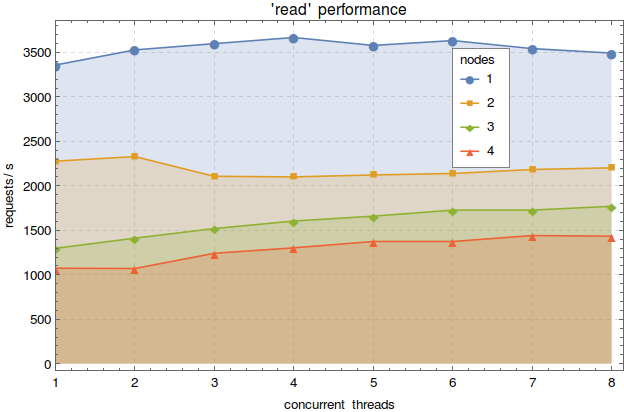
\includegraphics[width=0.8\textwidth]{images/fig04-benchmark.png}
	\caption[Pomiar wydajności w funkcji liczby współbieżnych operacji.]{Pomiar wydajności w funkcji liczby współbieżnych operacji. Pomiary wynonano z wyłączeniem operacji I/O będących wąskim gardłem.  Wszystkie węzły działają na \textbf{jednej} maszynie.}
	\label{fig:benchmark}
\end{figure}

\subsection{Wnioski}

Uruchamiając pojedynczy węzeł systemu na współczesnym laptopie\footnote{CPU: i5-4200u, Intel Haswell, 2C/4T, 1.6-2.6GHz; SSD: Lite-On L3-N2128}, można przetworzyć nawet do około 4000 zapytań w ciągu sekundy. Należy pamiętać że jest to \textit{czysta} wydajność, tj. wydajność logiki systemu z minimalizacją wpływu czynników zewnętrznych (wyłączone operacje na fizycznych plikach i baza danych pracująca w trybie in-memory).

Analizując \autoref{fig:benchmark}, widać, że wraz z dokładaniem kolejnych węzłów wydajność systemu spada. Jest to naturalny wynik obsługi zapytań rozgłaszanych po całym systemie, gdzie wzrasta liczba odbiorców komunikatu. Ze wzrostem liczby węzłów spadek wydajności jest jednak coraz mniejszy. Ponadto, już w przypadku plików o rozmiarze kilku megabajtów, ograniczenie wydajności przez wydajność dysku maszyny sprawiało, że spadek związany z wzrostem ilości węzłów jest całkowicie pomijalny.

Druga ważna obserwacja to \textit{współbieżność} systemu. Rozkładając zapytania na wiele wątków (wielu użytkowników korzystających z systemu), sumaryczna liczba przetworzonych zapytań będzie zgodnie z oczekiwaniami większa. Zrównoleglenie operacji odbywa się na dwóch poziomach: rozkładaniu zapytań na poszczególne węzły systemu oraz współbieżne przetwarzanie przez wątki wykonawcze węzła.

Stopień optymalizacji dostępu do zasobów z uwzględnieniem profilu użytkownika jest trudny do zmierzenia oraz do jednoznacznej oceny. Wprowadzenie do procesu przetwarzania zapytań warstwy dodatkowej logiki, odpowiedzialnej za szeregowanie zadań ma zgodnie z oczekiwaniami negatywny wpływ na bezwzględną wydajność wyrażoną jako liczba zapytań przetworzonych w jednostce czasu. Niestety, tylko taką wydajność w łatwy sposób można zmierzyć przy użyciu syntetycznych testów przeprowadzanych w sztucznym, symulowanym środowisku.

Obecne rozwiązanie dokonuje jedynie \textbf{klasyfikacji typu użytkownika}. Na podstawie historii operacji wyznaczane są parametry określające stosunek liczby zapisów do liczby odczytów oraz średni rozmiar plików na jakich operuje użytkownik. Pozwala to za zaklasyfikowanie go do różnych typów względem dwóch atrybutów:
\begin{itemize}
	\item \textit{typ}
	\begin{itemize}
		\item \textit{pisarz} - użytkownik  w przeważającej części dokonujący zapisów, czytający niewiele lub nic. Przykładem takiego użytkownika może być skrypt umieszczający w bazie danych pliki z odczytami pochodzącymi z urządzenia urządzenia pomiarowego w ośrodku badawczym.
		\item \textit{czytelnik} - użytkownik charakteryzujący się dużą liczbą częstych odczytów, mało zapisujący. Przykładowo może to być użytkownik przeglądający archiwalny katalog pomiarów.
		\item \textit{inny} - użytkownik równie często piszący co czytający.
	\end{itemize}
	\item \textit{waga}
	\begin{itemize}
		\item \textit{użytkownik lekki} - użytkownik często zapisujący i czytający małe pliki, przykłądowo tymczasowe wyniki obliczeń.
		\item \textit{użytkownik ciężki} - użytkownik dokonujący operacji na bardzo dużych plikach, na przykład archiwizujący duże zbiory danych.
	\end{itemize}
\end{itemize}

W zależności od przeznaczenia klastra z instalacją systemu, zapytania różnych użytkowników mogą mieć przydzielony różny priorytet. Takie priorytety można ustalić w module schedulera. Przykładowo, w instytucji może być potrzebny klaster storage'owy do którego urządzenia bezpośrednio zapisują wyniki pomiarów, oraz klaster służący do archiwizacji tych danych, po uprzednim przetworzeniu ich przez ludzkich użytkowników.

W celu ilościowego oszacowania wpływu schedulera na efektywność działania systemu, należałoby:
\begin{itemize}
	\item wprowadzić nową metrykę, wyrażającą \textit{zadowolenie} użytkowników (ang. \textit{happiness}) w formalny, liczbowy sposób. Różne ustawienia zapytań w kolejce schedulera powinny dawać różną wartość w tej metryce (\textit{funkcja celu}).
	\item opracować sposób maksymalizacji funkcji celu (zadowolenia) z użyciem optymalizacyjnych metod heurystycznych i algorytmów genetycznych \cite{genetic-wiki}.
	\item przygotować zestaw operacji symulujących różne typy użytkowników do użycia w testach wydajnościowych.
\end{itemize}

\subsection{Propozycje dalszych prac}

Nie udało się jeszcze wykonać testów w "prawdziwym" środowisku do jakiego system jest przeznaczony, czyli na zbiorze maszyn połączonych w sieć lokalną. Kolejnym etapem w pracach mogłoby być więc przygotowani kilku fizycznych maszyn połączonych w LAN na których uruchomionoby instancję systemu. Prawdopodobnie spadek wydajności związany z dokładaniem kolejnych węzłów będzie znacznie mniejszy - węzły będą działać na osobnych maszynach. Należy jednak pamiętać że wykorzystanie o wiele bardziej skomplikowanego stosu sieciowego może mieć negatywny wpływ na wydajność. Kolejnym ograniczeniem będzie limit prędkości transmisji plików.

Prezentowany system był pierwszą dużą rozproszoną aplikacją autorów. Z obecnego punktu widzenia wiele rzeczy zostałoby rozwiązanych inaczej. Być może nabyte doświadczenie zostanie wykorzystane w przyszłości do budowy nowego systemu o rozszerzonej funkcjonalności, bazującego na obecnym projekcie, powielającego dobre rozwiązania i kładącego większy nacisk na te, które  wymagają usprawnienia - precyzyjne sformułowanie SLA, lepszą skalowalność horyzontalną i poprawione algorytmy szeregowania zadań.
